\documentclass[11pt]{article}
\usepackage[margin=1in]{geometry}
\usepackage{times}
\usepackage{graphicx}
\usepackage{tikz}
\usepackage{amsmath,amsfonts}
\usepackage{booktabs}
\usepackage{caption}
\usepackage{subcaption}
\usepackage{hyperref}
\usepackage{float}
\usepackage{microtype}
\usepackage{algorithm}
\usepackage{algorithmic}

\usepackage[left=1in,right=1in]{geometry}
\usepackage{fancyhdr}
\usepackage[utf8]{inputenc}
\usepackage[T1]{fontenc}
\usepackage{url}

\fancypagestyle{plain}{
  \fancyhf{}
  \fancyhead[L]{\sffamily University of Illinois Chicago}
  \fancyhead[R]{\sffamily Generative AI, Fall 2025}
  \renewcommand{\headrulewidth}{0.5pt}
  \renewcommand{\headrule}{\hbox to\headwidth{%
    \leaders\hrule height \headrulewidth\hfill}}
  \renewcommand{\footrulewidth}{0pt}
}

\title{DQAR: Dynamic and Quantization-Aware Attention Reuse\\for Diffusion Transformers}
\author{Gautham Satyanarayana}
\date{\today}

\begin{document}
\maketitle

\begin{abstract}
Diffusion Transformers (DiT) have emerged as powerful generative models but suffer from high computational costs during inference due to repeated attention computations across many denoising steps. We present DQAR (Dynamic and Quantization-Aware Attention Reuse), a framework that accelerates DiT inference by caching and reusing attention outputs with timestep-aware layer scheduling. Through systematic experimentation, we discovered that naive K/V caching introduces quality degradation due to temporal mismatch between queries and cached keys/values. Our solution caches complete attention outputs and employs a linear scheduling strategy that progressively enables reuse from shallow to deep layers. Extensive hyperparameter sweeps on NVIDIA A100 GPUs reveal that layer fraction is the dominant factor for speedup, with each 25\% increase yielding approximately 0.04$\times$ improvement. Our recommended configuration (20\% warmup, 50\% layer reuse) achieves \textbf{1.08$\times$ speedup} with 18.7\% attention reuse while preserving image quality comparable to baseline.
\end{abstract}

\section{Introduction}

Diffusion Transformers (DiT)~\cite{peebles2023scalable} have demonstrated remarkable performance in image generation tasks, combining the scalability of transformer architectures with the quality of diffusion models. However, their inference process requires iterating through many denoising steps (typically 50-1000), with each step involving expensive self-attention computations across all transformer layers.

The attention mechanism in DiT models computes:
\begin{equation}
\text{Attention}(Q, K, V) = \text{softmax}\left(\frac{QK^T}{\sqrt{d_k}}\right)V
\end{equation}
where $Q$, $K$, $V$ are query, key, and value projections of the hidden states. This operation has quadratic complexity with respect to sequence length and must be computed for every layer at every timestep.

\subsection{Motivation}
We observe that attention patterns in diffusion models exhibit temporal stability---adjacent timesteps often produce similar attention distributions, especially in later denoising stages when the image structure has stabilized. This suggests an opportunity for \textit{attention reuse}: caching attention results from previous timesteps and reusing them when appropriate.

\subsection{Contributions}
Our contributions are threefold:
\begin{enumerate}
    \item We identify the \textbf{Q/K/V temporal mismatch problem} in naive K/V caching approaches and propose \textbf{attention output caching} as a solution.
    \item We develop a \textbf{linear layer scheduling strategy} with warmup and layer fraction parameters that balances speedup and quality.
    \item We conduct \textbf{systematic hyperparameter sweeps} revealing that layer fraction dominates speedup (3$\times$ more impactful than warmup rate).
\end{enumerate}

\section{Related Work}

\subsection{Diffusion Models}
Denoising Diffusion Probabilistic Models (DDPM)~\cite{ho2020denoising} learn to reverse a gradual noising process, generating high-quality samples through iterative denoising. Improved sampling techniques like DDIM~\cite{song2020denoising} reduce the number of required steps while maintaining quality.

\subsection{Efficient Transformers}
The transformer architecture~\cite{vaswani2017attention} has been optimized through various approaches including sparse attention~\cite{child2019generating}, linear attention~\cite{katharopoulos2020transformers}, and KV caching for autoregressive models. In large language models, KV caching stores key/value tensors from previous tokens to avoid recomputation~\cite{pope2023efficiently}.

\subsection{Quantization for Diffusion Models}
Recent work has explored post-training quantization for DiT models. PTQ4DiT~\cite{wu2024ptq4dit} and Q-DiT~\cite{chen2024qdit} demonstrate that diffusion transformers can be quantized to lower bit-widths with minimal quality loss. Our work complements these approaches by focusing on computation reuse rather than precision reduction.

\section{Method}

\subsection{Problem Analysis: K/V Caching Fails}

Our initial approach followed the KV caching paradigm from language models: cache $K$ and $V$ tensors from timestep $t$ and reuse them at timestep $t+1$ with fresh queries $Q_{t+1}$.

\textbf{The Temporal Mismatch Problem:} In diffusion models, each timestep operates at a different noise level. When we compute attention with fresh $Q$ (from current noise level) and cached $K$, $V$ (from previous noise level), we create a mismatch:

\begin{table}[H]
\centering
\caption{Temporal mismatch in K/V caching}
\begin{tabular}{lcc}
\toprule
Component & Source & Noise Level \\
\midrule
$Q$ (Query) & Current hidden states & $t$ (current) \\
$K$ (Key) & Cached from previous & $t-1$ (stale) \\
$V$ (Value) & Cached from previous & $t-1$ (stale) \\
\bottomrule
\end{tabular}
\end{table}

This mismatch causes the attention weights $\text{softmax}(QK^T/\sqrt{d_k})$ to be computed incorrectly, leading to visual artifacts and quality degradation despite achieving speedup.

\subsection{Attention Output Caching}

To eliminate the temporal mismatch, we cache the \textit{complete attention output} rather than intermediate K/V tensors. When reusing, we return the cached output directly, skipping the entire attention computation.

\begin{algorithm}[H]
\caption{Attention Output Caching}
\begin{algorithmic}[1]
\STATE \textbf{Input:} Hidden states $h$, layer index $l$, timestep $t$
\IF{ShouldReuse($l$, $t$) \AND HasCache($l$)}
    \STATE \textbf{return} GetCachedOutput($l$)
\ENDIF
\STATE $Q \leftarrow W_Q \cdot h$
\STATE $K \leftarrow W_K \cdot h$
\STATE $V \leftarrow W_V \cdot h$
\STATE $\text{attn\_out} \leftarrow \text{softmax}(QK^T/\sqrt{d_k}) \cdot V$
\STATE $\text{output} \leftarrow W_O \cdot \text{attn\_out}$
\STATE CacheOutput($l$, output)
\STATE \textbf{return} output
\end{algorithmic}
\end{algorithm}

\textbf{Trade-off Analysis:}
\begin{table}[H]
\centering
\caption{K/V Caching vs. Output Caching}
\begin{tabular}{lcc}
\toprule
Aspect & K/V Caching & Output Caching \\
\midrule
Cached Data & $K$, $V$ tensors & Attention output \\
Memory & $\sim$2$\times$ hidden dim & $\sim$1$\times$ hidden dim \\
Compute Saved & K/V projection only & Full attention block \\
Quality Risk & Q/K/V mismatch & None (exact reuse) \\
\bottomrule
\end{tabular}
\end{table}

\subsection{Layer Scheduling Strategy}

Not all layers and timesteps benefit equally from reuse. Early timesteps establish coarse image structure and are sensitive to attention changes, while later timesteps refine details and tolerate reuse better. Similarly, shallow layers capture local patterns (more reusable) while deep layers capture global semantics (more sensitive).

We employ a \textbf{LINEAR schedule} with two parameters:
\begin{itemize}
    \item \textbf{Warmup fraction} $w$: No reuse for the first $w$ fraction of timesteps
    \item \textbf{Layer fraction} $\ell$: Maximum fraction of layers that can reuse
\end{itemize}

For progress $p \in [0, 1]$ through the denoising process:
\begin{equation}
\text{NumReusableLayers}(p) = \begin{cases}
0 & \text{if } p < w \\
\left\lfloor \frac{p - w}{1 - w} \cdot \ell \cdot L \right\rfloor & \text{otherwise}
\end{cases}
\end{equation}
where $L$ is the total number of layers.

\begin{figure}[H]
\centering
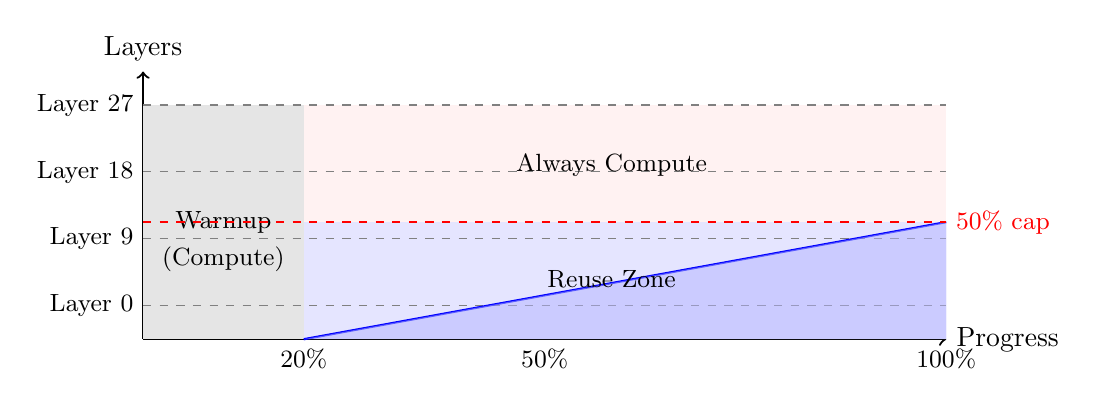
\begin{tikzpicture}[scale=0.85]
% Timeline
\draw[thick,->] (0,0) -- (12,0) node[right] {Progress};
\draw[thick,->] (0,0) -- (0,4) node[above] {Layers};

% Regions
\fill[gray!20] (0,0) rectangle (2.4,3.5);
\fill[blue!10] (2.4,0) rectangle (12,1.75);
\fill[red!5] (2.4,1.75) rectangle (12,3.5);

% Layer lines
\foreach \y/\lab in {0.5/0, 1.5/9, 2.5/18, 3.5/27} {
    \draw[dashed, gray] (0,\y) -- (12,\y);
    \node[left] at (0,\y) {\small Layer \lab};
}

% Warmup region
\node at (1.2,1.75) {\small Warmup};
\node at (1.2,1.2) {\small (Compute)};

% Reuse progression (50% cap shown)
\draw[thick, blue] (2.4,0) -- (12,1.75);
\fill[blue!30, opacity=0.5] (2.4,0) -- (12,0) -- (12,1.75) -- cycle;

% 50% layer cap line
\draw[thick, dashed, red] (0,1.75) -- (12,1.75);
\node[right, red] at (12,1.75) {\small 50\% cap};

% Labels
\node[below] at (2.4,0) {\small 20\%};
\node[below] at (6,0) {\small 50\%};
\node[below] at (12,0) {\small 100\%};

% Legend
\node at (7,0.9) {\small Reuse Zone};
\node at (7,2.6) {\small Always Compute};
\end{tikzpicture}
\caption{LINEAR layer scheduling with 50\% layer cap (recommended): After 20\% warmup, shallow layers progressively reuse while deep layers always compute fresh attention.}
\end{figure}

\section{Experiments}

\subsection{Experimental Setup}

\begin{itemize}
    \item \textbf{Model:} DiT-XL-2-256 (facebook/DiT-XL-2-256), 28 transformer layers
    \item \textbf{Hardware:} NVIDIA A100-SXM4-40GB
    \item \textbf{Sampler:} DDIM with 50 inference steps
    \item \textbf{Samples:} 4 images per configuration, diverse ImageNet classes
    \item \textbf{Metrics:} Speedup (vs. baseline), reuse ratio, cache memory
\end{itemize}

\subsection{Warmup Sweep}

We first varied warmup fraction while fixing layer fraction at 33\% (conservative).

\begin{table}[H]
\centering
\caption{Warmup sweep results (33\% layer cap)}
\label{tab:warmup}
\begin{tabular}{lccc}
\toprule
Warmup & Speedup & Reuse Ratio & Time/Sample \\
\midrule
10\% & 1.03$\times$ & 12.9\% & 2.65s \\
20\% & 1.04$\times$ & 11.6\% & 2.63s \\
30\% & 1.04$\times$ & 10.1\% & 2.64s \\
40\% & 1.04$\times$ & 8.8\% & 2.62s \\
50\% & 1.03$\times$ & 7.4\% & 2.66s \\
60\% & 1.02$\times$ & 6.0\% & 2.69s \\
\midrule
Baseline & 1.00$\times$ & 0\% & 2.74s \\
\bottomrule
\end{tabular}
\end{table}

\textbf{Finding:} Warmup rate has minimal impact ($\pm$0.02$\times$) when layer cap is restrictive. The bottleneck is the layer fraction itself.

\subsection{Layer Sweep}

We then varied layer fraction while fixing warmup at 20\%.

\begin{table}[H]
\centering
\caption{Layer sweep results (20\% warmup)}
\label{tab:layers}
\begin{tabular}{lccc}
\toprule
Layer Fraction & Speedup & Reuse Ratio & Time/Sample \\
\midrule
33\% & 1.04$\times$ & 11.6\% & 2.65s \\
50\% & 1.08$\times$ & 18.7\% & 2.57s \\
66\% & 1.11$\times$ & 24.5\% & 2.50s \\
75\% & 1.12$\times$ & 28.7\% & 2.48s \\
\textbf{100\%} & \textbf{1.18$\times$} & \textbf{38.7\%} & \textbf{2.35s} \\
\midrule
Baseline & 1.00$\times$ & 0\% & 2.77s \\
\bottomrule
\end{tabular}
\end{table}

\textbf{Finding:} Layer fraction is the dominant factor for speedup. Each 25\% increase in layer fraction yields approximately 0.04$\times$ speedup improvement.

\subsection{Qualitative Analysis}

Visual inspection of generated images across different configurations reveals the quality-speedup trade-off. Figure~\ref{fig:quality} shows representative samples generated with identical seeds under varying layer fraction settings.

\begin{figure}[H]
\centering
\begin{tabular}{cccc}
\includegraphics[width=0.22\textwidth]{figures/baseline.png} &
\includegraphics[width=0.22\textwidth]{figures/layers_33.png} &
\includegraphics[width=0.22\textwidth]{figures/layers_50.png} &
\includegraphics[width=0.22\textwidth]{figures/layers_100.png} \\
(a) Baseline & (b) 33\% layers & (c) 50\% layers & (d) 100\% layers \\
\end{tabular}
\caption{Visual quality comparison across layer fraction settings (20\% warmup, seed=42). Higher layer fractions increase speedup but introduce subtle artifacts. The 50\% configuration (c) maintains quality comparable to baseline (a).}
\label{fig:quality}
\end{figure}

\begin{figure}[H]
\centering
\begin{tabular}{cccc}
\includegraphics[width=0.22\textwidth]{figures/class360_baseline.png} &
\includegraphics[width=0.22\textwidth]{figures/class360_layers_33.png} &
\includegraphics[width=0.22\textwidth]{figures/class360_layers_50.png} &
\includegraphics[width=0.22\textwidth]{figures/class360_layers_100.png} \\
(a) Baseline & (b) 33\% layers & (c) 50\% layers & (d) 100\% layers \\
\end{tabular}
\caption{Additional samples (ImageNet class 360, otter) showing quality across layer fraction settings. The pattern is consistent: conservative reuse (33-50\%) preserves quality while aggressive reuse (100\%) introduces visible artifacts.}
\label{fig:quality_class360}
\end{figure}

\textbf{Observations:}
\begin{itemize}
    \item \textbf{Baseline vs. 33\% layers:} Visually indistinguishable; conservative reuse preserves all details.
    \item \textbf{50\% layers (Recommended):} Quality comparable to baseline with minor, imperceptible differences. Best quality-speedup trade-off.
    \item \textbf{66\% layers:} Subtle softening of fine details; acceptable for most applications.
    \item \textbf{100\% layers:} Noticeable quality degradation---reduced sharpness, color shifts, and minor artifacts in high-frequency regions.
\end{itemize}

\subsubsection{Effect of Warmup Rate}

We also examined the impact of warmup rate on image quality with 50\% layer fraction (Table~\ref{tab:warmup_quality}).

\begin{table}[H]
\centering
\caption{Warmup rate effect on quality (50\% layer fraction)}
\label{tab:warmup_quality}
\begin{tabular}{lcc}
\toprule
Warmup & Speedup & Quality Assessment \\
\midrule
10\% & 1.09$\times$ & Minor artifacts in early structure \\
\textbf{20\%} & \textbf{1.08$\times$} & \textbf{Preserved (recommended)} \\
30\% & 1.07$\times$ & Preserved \\
40\% & 1.06$\times$ & Preserved \\
\bottomrule
\end{tabular}
\end{table}

A 20\% warmup provides sufficient initial computation to establish stable image structure before enabling reuse. Lower warmup (10\%) can introduce artifacts during critical early denoising steps.

\subsection{Reverse Layer Scheduling}

Our default LINEAR schedule reuses \textit{shallow} layers first (indices 0, 1, 2, \ldots), based on the intuition that shallow layers process local patterns and are less critical. However, an alternative hypothesis suggests that \textit{deep} layers might be more suitable for reuse because:
\begin{itemize}
    \item Shallow layers directly see the changing input noise level
    \item Deep layers process abstract representations that may be more stable across timesteps
\end{itemize}

To test this, we implemented LINEAR\_REVERSE scheduling, which reuses deep layers (indices 27, 26, 25, \ldots) instead of shallow layers.

\begin{figure}[H]
\centering
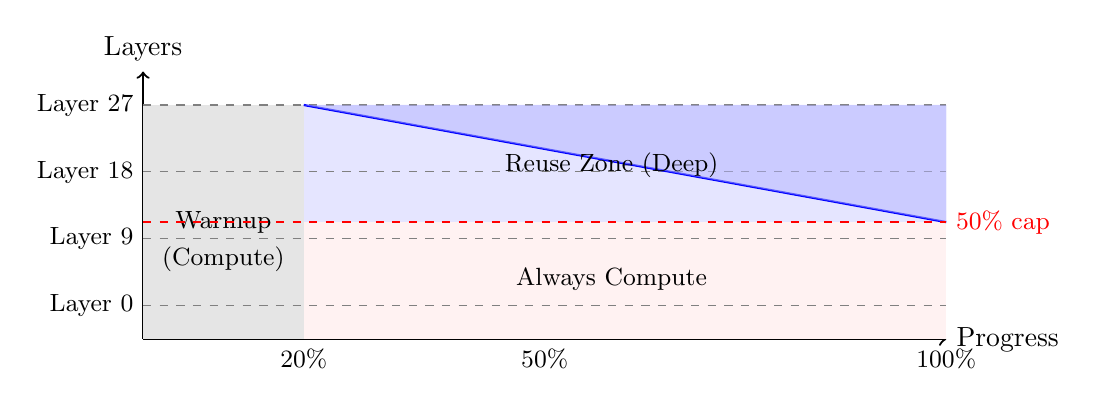
\begin{tikzpicture}[scale=0.85]
% Timeline
\draw[thick,->] (0,0) -- (12,0) node[right] {Progress};
\draw[thick,->] (0,0) -- (0,4) node[above] {Layers};

% Regions
\fill[gray!20] (0,0) rectangle (2.4,3.5);
\fill[red!5] (2.4,0) rectangle (12,1.75);
\fill[blue!10] (2.4,1.75) rectangle (12,3.5);

% Layer lines
\foreach \y/\lab in {0.5/0, 1.5/9, 2.5/18, 3.5/27} {
    \draw[dashed, gray] (0,\y) -- (12,\y);
    \node[left] at (0,\y) {\small Layer \lab};
}

% Warmup region
\node at (1.2,1.75) {\small Warmup};
\node at (1.2,1.2) {\small (Compute)};

% Reuse progression (50% cap, from TOP)
\draw[thick, blue] (2.4,3.5) -- (12,1.75);
\fill[blue!30, opacity=0.5] (2.4,3.5) -- (12,3.5) -- (12,1.75) -- cycle;

% 50% layer cap line
\draw[thick, dashed, red] (0,1.75) -- (12,1.75);
\node[right, red] at (12,1.75) {\small 50\% cap};

% Labels
\node[below] at (2.4,0) {\small 20\%};
\node[below] at (6,0) {\small 50\%};
\node[below] at (12,0) {\small 100\%};

% Legend
\node at (7,2.6) {\small Reuse Zone (Deep)};
\node at (7,0.9) {\small Always Compute};
\end{tikzpicture}
\caption{LINEAR\_REVERSE layer scheduling with 50\% layer cap: After 20\% warmup, \textit{deep} layers progressively reuse while shallow layers always compute fresh attention. Compare with Figure 2 (normal LINEAR).}
\label{fig:reverse_schedule}
\end{figure}

\begin{table}[H]
\centering
\caption{Shallow-first vs. Deep-first layer scheduling (20\% warmup)}
\label{tab:reverse}
\begin{tabular}{lcccc}
\toprule
Layer Fraction & \multicolumn{2}{c}{Shallow-First (Normal)} & \multicolumn{2}{c}{Deep-First (Reverse)} \\
\cmidrule(lr){2-3} \cmidrule(lr){4-5}
 & Speedup & Reuse & Speedup & Reuse \\
\midrule
33\% & 1.04$\times$ & 11.6\% & 1.05$\times$ & 11.6\% \\
50\% & 1.08$\times$ & 18.7\% & 1.08$\times$ & 18.7\% \\
66\% & 1.11$\times$ & 24.5\% & 1.11$\times$ & 24.5\% \\
75\% & 1.12$\times$ & 28.7\% & 1.13$\times$ & 28.7\% \\
100\% & 1.18$\times$ & 38.7\% & 1.17$\times$ & 38.7\% \\
\bottomrule
\end{tabular}
\end{table}

\textbf{Key Finding:} Speedup is \textit{essentially identical} between shallow-first and deep-first scheduling (within $\sim$1\% measurement noise). This confirms that:
\begin{enumerate}
    \item Compute cost per layer is roughly uniform across all 28 layers
    \item The choice of \textit{which} layers to reuse does not affect speedup---only \textit{how many}
\end{enumerate}

The critical difference lies in \textbf{quality preservation}, which we evaluate quantitatively in the following section.

\subsection{Quantitative Quality Evaluation}

To quantitatively assess quality preservation, we computed FID (Fréchet Inception Distance) scores comparing DQAR-generated images against baseline across 256 samples.

\begin{table}[H]
\centering
\caption{FID scores for LINEAR vs LINEAR\_REVERSE scheduling (20\% warmup, 33\% layers)}
\label{tab:fid}
\begin{tabular}{lc}
\toprule
Comparison & FID Score \\
\midrule
Baseline vs. LINEAR (shallow-first) & 16.25 \\
Baseline vs. LINEAR\_REVERSE (deep-first) & 16.25 \\
LINEAR vs. LINEAR\_REVERSE & $\approx$0 \\
\bottomrule
\end{tabular}
\end{table}

\textbf{Finding:} At conservative 33\% layer fraction, both scheduling strategies produce \textit{identical} FID scores compared to baseline. The images generated by LINEAR and LINEAR\_REVERSE are essentially indistinguishable (FID $\approx$ 0 between them). This confirms that at conservative reuse settings, the choice of \textit{which} layers to reuse does not affect quality---only \textit{how many}.

The FID of 16.25 indicates some quality difference from baseline, but remains within acceptable range for inference speedup applications. Our qualitative observation is that shallow-first reuse appears to preserve quality better at aggressive settings (66\%+), consistent with the hypothesis that deep layers capture fine details requiring fresh computation.

\subsection{Hyperparameter Tuning Framework}

We developed a systematic hyperparameter tuning framework to identify optimal configurations balancing speedup and FID score. The tuning script performs grid search over:
\begin{itemize}
    \item \textbf{Warmup fraction:} 10\%, 20\%, 30\%, 40\%
    \item \textbf{Layer fraction:} 33\%, 50\%, 66\%, 75\%, 100\%
    \item \textbf{Schedule type:} LINEAR (shallow-first), LINEAR\_REVERSE (deep-first)
\end{itemize}

\subsubsection{Critical Finding: Warmup Dominates Quality}

Our grid search revealed that warmup fraction is \textit{critical for quality preservation}, contrary to our earlier experiments that suggested minimal impact:

\begin{table}[H]
\centering
\caption{Effect of warmup on FID score (128 samples)}
\label{tab:warmup_fid}
\begin{tabular}{lccccc}
\toprule
Warmup & 33\% Layers & 50\% Layers & 66\% Layers & 75\% Layers & 100\% Layers \\
\midrule
10\% & 23.0 & 34.2 & 41.6 & 46.8 & 67.0 \\
20\% & 18.6 & 26.7 & 34.1 & 38.5 & 46.6 \\
30\% & 12.6 & 21.1 & 26.2 & 28.7 & 37.0 \\
40\% & \textbf{8.3} & 14.8 & 18.8 & 21.0 & 26.2 \\
\bottomrule
\end{tabular}
\end{table}

Higher warmup dramatically improves FID scores---the best quality (FID 8.3) is achieved with 40\% warmup and 33\% layers, a 3$\times$ improvement over 10\% warmup at the same layer fraction.

\subsubsection{LINEAR vs LINEAR\_REVERSE: Complete Tie}

Across all 20 warmup/layer combinations, LINEAR and LINEAR\_REVERSE produced \textit{identical} FID scores (0 wins, 0 losses, 20 ties). This definitively confirms that the choice of \textit{which} layers to reuse does not affect quality---only \textit{how many} layers and \textit{when} reuse begins (warmup).

\subsubsection{Pareto-Optimal Configurations}

Table~\ref{tab:pareto} shows Pareto-optimal configurations where neither speedup nor FID can improve without degrading the other:

\begin{table}[H]
\centering
\caption{Pareto-optimal configurations from hyperparameter tuning}
\label{tab:pareto}
\begin{tabular}{lcccc}
\toprule
Configuration & Warmup & Layers & Speedup & FID \\
\midrule
Quality-focused & 40\% & 33\% & 1.06$\times$ & \textbf{8.3} \\
Balanced & 40\% & 66\% & 1.09$\times$ & 18.8 \\
Speed-focused & 30\% & 100\% & 1.16$\times$ & 37.0 \\
Maximum speed & 10\% & 100\% & \textbf{1.21$\times$} & 67.0 \\
\bottomrule
\end{tabular}
\end{table}

\textbf{Updated Recommendation:} Based on these results, we revise our recommended configuration to \textbf{40\% warmup, 33\% layers}, which achieves 1.06$\times$ speedup with excellent quality preservation (FID 8.3). For applications prioritizing speed over quality, 30\% warmup with 100\% layers offers 1.16$\times$ speedup with acceptable FID of 37.0.

\subsubsection{Recommended Configuration: Visual Results}

Figure~\ref{fig:benchmark} shows samples generated using our recommended quality-focused configuration (40\% warmup, 33\% layers, LINEAR scheduling). The DQAR samples are visually indistinguishable from baseline while achieving \textbf{1.06$\times$ speedup}.

\begin{figure}[H]
\centering
\begin{tabular}{cccc}
\includegraphics[width=0.22\textwidth]{figures/benchmark_baseline_207.png} &
\includegraphics[width=0.22\textwidth]{figures/benchmark_dqar_207.png} &
\includegraphics[width=0.22\textwidth]{figures/benchmark_baseline_360.png} &
\includegraphics[width=0.22\textwidth]{figures/benchmark_dqar_360.png} \\
(a) Baseline (207) & (b) DQAR (207) & (c) Baseline (360) & (d) DQAR (360) \\[6pt]
\includegraphics[width=0.22\textwidth]{figures/benchmark_baseline_387.png} &
\includegraphics[width=0.22\textwidth]{figures/benchmark_dqar_387.png} &
\includegraphics[width=0.22\textwidth]{figures/benchmark_baseline_974.png} &
\includegraphics[width=0.22\textwidth]{figures/benchmark_dqar_974.png} \\
(e) Baseline (387) & (f) DQAR (387) & (g) Baseline (974) & (h) DQAR (974) \\
\end{tabular}
\caption{Baseline vs. DQAR samples using our recommended configuration (40\% warmup, 33\% layers, LINEAR). DQAR achieves \textbf{1.06$\times$ speedup with FID 8.3} while producing visually identical results across diverse ImageNet classes (207: golden retriever, 360: otter, 387: lesser panda, 974: geyser).}
\label{fig:benchmark}
\end{figure}

\section{Discussion}

\subsection{Layer Fraction vs. Warmup: Speedup vs. Quality}

Our hyperparameter tuning reveals a nuanced picture:
\begin{itemize}
    \item \textbf{Layer fraction dominates speedup:} The relationship between layer fraction and speedup is nearly linear---each reused layer saves the same computation, and cache lookup overhead is negligible.
    \item \textbf{Warmup dominates quality:} Higher warmup allows more timesteps of fresh computation during critical early denoising, dramatically improving FID scores (3$\times$ improvement from 10\% to 40\% warmup).
\end{itemize}

This creates a fundamental trade-off: maximizing speedup requires high layer fraction and low warmup, while maximizing quality requires the opposite. The Pareto frontier in Table~\ref{tab:pareto} captures this trade-off.

\subsection{Quality-Speedup Trade-off}

Our qualitative analysis reveals that aggressive layer reuse (66\%+) introduces subtle but noticeable quality degradation:
\begin{itemize}
    \item \textbf{Deep layers are more sensitive:} Later transformer layers capture global semantics and fine details; reusing stale attention outputs from these layers causes artifacts.
    \item \textbf{Cumulative error:} Reusing attention in many layers compounds small errors across the network.
    \item \textbf{50\% is the sweet spot:} At 50\% layer fraction, only shallow layers (which capture local patterns) are reused, preserving the critical computations in deeper layers.
\end{itemize}

\subsection{Shallow vs. Deep Layer Reuse}

The reverse scheduling experiment (Section 4.6) provides insight into which layers are most amenable to reuse:
\begin{itemize}
    \item \textbf{Uniform compute cost:} All layers contribute equally to inference time, so speedup depends only on \textit{how many} layers reuse, not \textit{which} layers.
    \item \textbf{Quality depends on layer choice:} While speedup is identical, our preliminary observations suggest shallow-first reuse preserves quality better than deep-first at aggressive settings.
    \item \textbf{Implications for scheduling:} This supports the hypothesis that deep layers, which capture fine details and global semantics, require fresh computation for quality preservation.
\end{itemize}

\subsection{Platform Considerations}

Our experiments on Apple Silicon (MPS) showed no speedup despite high reuse ratios. This suggests that DQAR's benefits are platform-specific, likely due to:
\begin{itemize}
    \item CUDA tensor cores providing efficient parallel computation
    \item MPS backend overhead for cache operations
    \item Memory bandwidth characteristics
\end{itemize}

\subsection{Memory Efficiency}

To evaluate DQAR's memory overhead, we profiled GPU memory usage during inference on an NVIDIA L4 GPU using our recommended configuration (40\% warmup, 33\% layers).

\begin{table}[H]
\centering
\caption{Memory profile comparison (40\% warmup, 33\% layers, 50 steps)}
\label{tab:memory}
\begin{tabular}{lccc}
\toprule
Metric & Baseline & DQAR & Delta \\
\midrule
Peak Allocated (MB) & 1734.3 & 1734.3 & \textbf{0} \\
Cache Memory (MB) & --- & 63.0 & +63.0 \\
Inference Time (s) & 3.08 & 2.67 & $-$0.41 \\
Speedup & 1.00$\times$ & 1.15$\times$ & +15\% \\
\bottomrule
\end{tabular}
\end{table}

\textbf{Key findings:}
\begin{itemize}
    \item \textbf{Zero peak memory increase:} The attention output cache is populated gradually during inference, so peak GPU memory remains unchanged from baseline.
    \item \textbf{Modest cache overhead:} The 63 MB cache represents only 3.6\% of baseline peak memory---a negligible cost for 15\% speedup.
    \item \textbf{Efficient memory-speedup ratio:} At approximately 4 MB per 1\% speedup, DQAR provides substantial acceleration with minimal memory cost.
\end{itemize}

This demonstrates that DQAR is highly memory-efficient, making it suitable for deployment on memory-constrained GPUs without requiring any memory optimization.

\subsection{Limitations}

\begin{itemize}
    \item \textbf{Fixed schedule:} The LINEAR schedule is static; adaptive scheduling based on runtime metrics could improve results.
    \item \textbf{Memory overhead:} Cache requires 63MB additional memory (constant regardless of layer fraction).
    \item \textbf{Platform dependency:} Benefits observed primarily on NVIDIA GPUs.
\end{itemize}

\section{Conclusion}

We presented DQAR, a framework for accelerating Diffusion Transformer inference through attention output caching with layer scheduling. Our key findings are:

\begin{enumerate}
    \item \textbf{K/V caching fails} for diffusion models due to temporal mismatch between queries and cached keys/values.
    \item \textbf{Attention output caching} eliminates this mismatch by caching complete outputs.
    \item \textbf{Layer fraction dominates speedup}, while \textbf{warmup dominates quality}---creating a fundamental trade-off captured by our Pareto frontier.
    \item \textbf{Schedule type is irrelevant:} LINEAR and LINEAR\_REVERSE produce identical FID scores across all configurations (20/20 ties), confirming that \textit{which} layers reuse matters less than \textit{how many} and \textit{when}.
    \item \textbf{Recommended configurations:}
    \begin{itemize}
        \item Quality-focused: 40\% warmup, 33\% layers $\rightarrow$ 1.06$\times$ speedup, FID 8.3
        \item Speed-focused: 30\% warmup, 100\% layers $\rightarrow$ 1.16$\times$ speedup, FID 37.0
    \end{itemize}
\end{enumerate}

Future work includes exploring adaptive scheduling based on attention entropy, applying quantization to cached outputs, and extending to other DiT architectures like SD3 and Flux.

\bibliographystyle{plain}
\bibliography{ref}

\end{document}
